\chapter{PERANCANGAN SISTEM}

Bab ini menjelaskan mengenai perancangan data dan sistem rancang bangun aplikasi pendeteksi daun berbasis Android. Bab ini juga akan menjelaskan gambaran umum sistem.

\section{Perancangan Data}
\par Data yang digunakan sebagai masukan awal dari sistem rancang bangun aplikasi pendeteksi daun berbasis Android adalah dataset yang dibuat Pedro F. B. Silva dan Andra Marasal menggunakan spesimen Rubim Almeida da Silva dari the Faculty of Science, University of Porto, Portugal. Dataset tersebut berisi 483 data yang terbagi dalam 40 kelas. 

\begin{figure}[ht]
	\begin{subfigure}{0.5\textwidth}
		\centering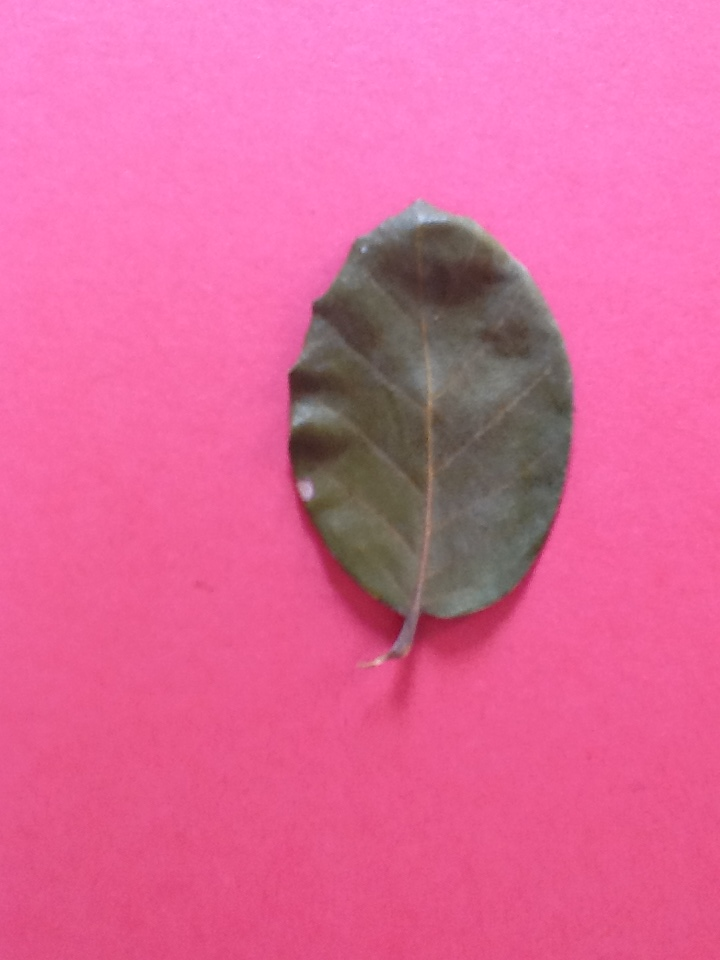
\includegraphics[width=\linewidth]{bab3/figures/quercus_suber.JPG}
		\caption{Quercus Suber}
		\label{fig:quercus_suber}
	\end{subfigure}
	~
	\begin{subfigure}{0.5\textwidth}
		\centering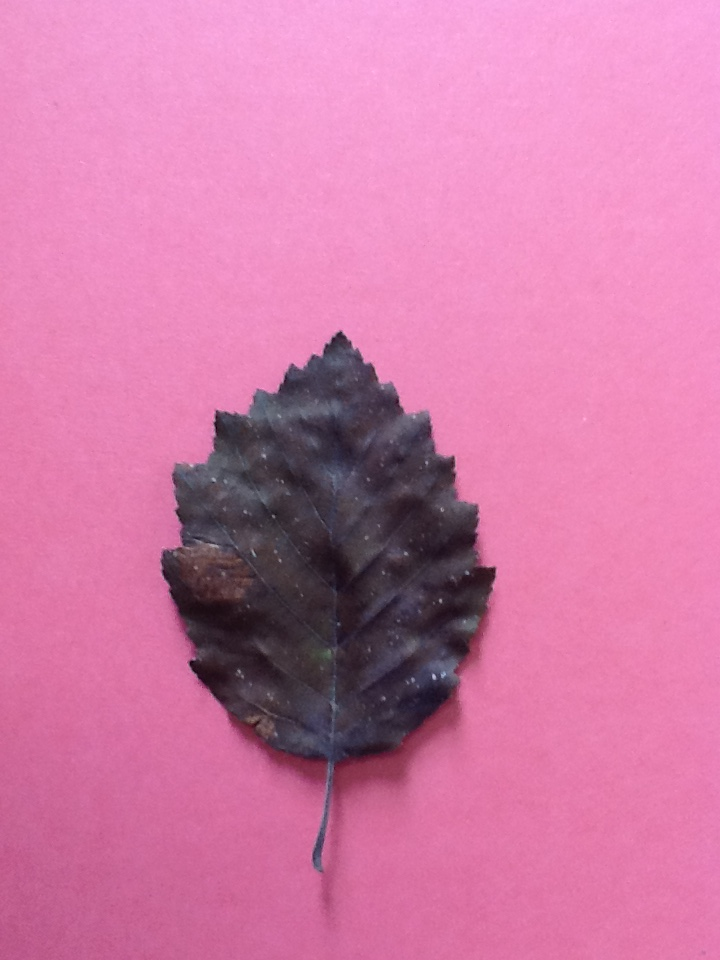
\includegraphics[width=\linewidth]{bab3/figures/alnus_sp.JPG}
		\caption{Alnus sp}
		\label{fig:alnus_sp}
	\end{subfigure}
	~
	\caption{Contoh gambar daun pada dataset}
\end{figure}

\par Dataset tersebut berisi gambar sehelai daun dengan background pink dan tidak ada benda lain di sekelilingnya. 

\par Selain dataset dari Pedro F. B. Silva dan Andra Marasal, penulis akan menambahkan dataset sendiri dengan daun-daun yang umum ditemukan di Indonesia. Adapun gambar-gambar yang akan ditambahkan penulis lebih tidak teratur dalam artian latar belakangnya bisa berwarna-warni dan mengandung noise.

\section{Desain Umum Sistem}
\par Desain umum dari sistem pendeteksi daun berbasis Android ini terdiri dari tiga bagian, yaitu tahap ekstraksi fitur, tahap pelatihan, dan aplikasi Android. 
\par Tahap ekstraksi fitur dilakukan paling awal dalam tahap membuat model. Gambar diekstraksi fiturnya dengan menggunakan arsitektur-arsitektur yang akan diuji dan dibandingkan. Setelah fitur-fitur pada gambar diekstraksi dan disimpan dalam file, dilakukan tahap pelatihan. 
\par Dengan tahap pelatihan, dibuatlah sebuah model atau \textit{classifier} yang akan dipakai untuk memprediksi daun yang diunggah ke-server.
\par Pengguna sendiri akan berinteraksi dengan perangkat lunak berbasis android yang memiliki beberapa fungsi, seperti prediksi, unggah dan latih. Aplikasi Android akan berperan sebagai perantara antara pengguna dan peladen.

\subsection{Tahap Ekstraksi Fitur}
\par Sistem dan model \textit{deep learning} adalah arsitektur berlapis yang mempelajari fitur yang berbeda pada layer yang berbeda (representasi hierarkis fitur berlapis). Layer-layer ini akhirnya terhubung ke lapisan terakhir (biasanya \textit{fully-connected layer}, untuk mendapatkan hasil akhir. Arsitektur berlapis ini memungkinkan kita untuk menggunakan jaringan yang sudah dilatih sebelumnya (seperti InceptionV3 atau VGG) tanpa layer terakhirnya sebagai ekstraktor fitur tetap untuk tugas-tugas lain.
\par Ini idealnya digunakan ketika data yang kita coba latih sangat mirip dengan pre-trained model dan ukuran dataset kecil.
\par Pada tahap awal dari ekstraksi fitur dilakukan praproses input menggunakan library Keras. Bobot pre-trained yang tersedia di Keras dilatih dengan langkah preproses yang didefinisikan dalam fungsi \textit{preprocess input} yang tersedia untuk setiap arsitektur jaringan (VGG16, InceptionV3, dll).
\par Setelah praproses dilakukan, akan dijalankan ekstraksi fitur dengan arsitektur jaringan tertentu. Setelah fitur diekstraksi, hasil ekstraksi fitur tersebut  akan di-\textit{flatten} sehingga membentuk array. Lalu setelah fitur dari semua gambar telah diekstraksi, datanya disimpan dalam file berekstensi h5. Label-label dari gambar-gambar tersebut juga akan disimpan dalam file berekstensi h5. File-file h5 ini akan digunakan dalam tahap selanjutnya yaitu pembuatan model.

\subsubsection{Ekstraksi Fitur dengan VGG16}
\par VGG16 merupakan arsitektur konvolusi pembelajaran dalam dengan bobot 16 layer, yang terdiri dari 12 \textit{Convolutional Layer}, 3 \textit{Fully-Connected Layer}, dan \textit{Softmax Layer}. Proses ekstraksi fitur ini dilakukan menggunakan metode FCN (Fully Convolutional Layer) VGG-16. Dimana nilai vector yang di dapatkan dari Ekstraksi Fitur dengan 13 \textit{Convolution Layer}, 5 \textit{Max Pooling Layer} yang telah diubah menjadi vector menggunakan fungsi Flatten akan dijadikan sebagai input atribut data untuk tahap pembentukkan model.

\subsubsection{Ekstraksi Fitur dengan VGG19}
\par VGG19 adalah arsitektur dengan bobot 19 layer, terdiri dari 16 Convolution Layer dan 5 Max Pooling Layer. Secara garis besar VGG19 mirip dengan VGG16. 

\subsubsection{Ekstraksi Fitur dengan MobileNet}
\par Arsitektur ini menggunakan \textit{depth-wise separable convolution}yang secara signifikan mengurangi jumlah parameter bila dibandingkan dengan jaringan dengan konvolusi normal dengan kedalaman yang sama dalam jaringan. Ini menghasilkan jaringan saraf yang dalam dan ringan. 
\par Pengurangan jumlah parameter secara signifikan mengurangi jumlah total operasi yang menguntungkan dalam aplikasi \textit{mobile} dengan daya komputasi yang lebih sedikit.

\subsubsection{Ekstraksi Fitur dengan ResNet50}
\par ResNet-50 adalah jaringan saraf convolutional yang dilatih pada lebih dari satu juta gambar dari basis data ImageNet. Jaringan ini memiliki kedalaman 50 lapisan dan dapat mengklasifikasikan gambar ke dalam 1000 kategori objek, seperti keyboard, mouse, pensil, dan banyak binatang. Akibatnya, jaringan telah mempelajari representasi fitur yang kaya untuk berbagai gambar. Jaringan memiliki ukuran input gambar 224x224.

\par ResNet menggunakan \textit{skip connection} untuk menambahkan output dari lapisan sebelumnya ke lapisan selanjutnya. Ini membantu mengurangi masalah gradien yang hilang dan memungkinkan untuk melakukan pembelajaran dalam dengan banyak layer.

\subsubsection{Ekstraksi Fitur dengan InceptionV3}
\par InceptionV3 merupakan arsitektur jaringan yang terdiri dari 48 layer. InceptionV3 juga dilatih menggunakan lebih dari sejuta gambar pada basis data ImageNet. Inception menumpuk konvolusi 5x5 menjadi dua konvolusi 3x3 untuk peningkatan performa.

\subsubsection{Ekstraksi Fitur dengan Xception}
\par Xception diusulkan oleh François Chollet sendiri, pencipta dan kepala pengelola Keras.Xception adalah perpanjangan dari arsitektur Inception yang menggantikan modul Inception standar dengan \textit{depth-wise convolution}. Xception menampilkan serialisasi terkecil dengan berat hanya 91MB.

\subsection{Tahap Pelatihan}
\par Apabila ekstraksi fitur dengan arsitektur yang dipilih telah selesai, saatnya untuk melakukan pelatihan. Pelatihan dilakukan untuk membangun model klasifikasi untuk mendeteksi daun. 
\par Pelatihan dimulai dengan membuka file-file hasil ekstraksi fitur. Kemudian dari data hasil ekstraksi fitur tersebut dipecah menjadi train dataset dan test dataset untuk validasi. Ukuran perbandingan dari data test dan data train dapat diatur di file konfigurasi. Setelah dilakukan penyesuaian atau fit antara data train dengan metode klasifikasi \textit{Logistic Regression}. Untuk setiap data test akan dilakukan prediksi yang kemudian dicatat hasil keseluruhannya pada file berekstensi txt.
\par Hasil dari pengujian model akan di evaluasi menggunakan variabel evaluasi precision, recall,dan f1-score. 

\subsection{Aplikasi Android}
\par Aplikasi Android ini dikembangkan dengan bahasa pemrograman Java dan \textit{Integrated Development Environment} Android Studio. Adapun aplikasi ini akan membutuhkan akses pada kamera ponsel dan internet untuk dijalankan. Untuk menjalankan kamera pada ponsel, akan digunakan library fotoapparat. Terdapat tiga fitur pada aplikasi Android, yaitu :
\begin {enumerate}
\item Upload
\par Pengguna dapat mengunggah foto-foto daun, untuk menambah dataset pada server. Dengan fitur ini diharapkan jumlah label dan dataset daun bertambah, yang meningkatkan kredibilitas aplikasi. 
\par Fitur upload akan menembak API pada server dengan parameter gambar daun yang telah diubah menjadi string serta nama daun.
\item Predict
\par Pengguna dapat mengunggah foto daun yang ingin dicari jenisnya. Server kemudian akan mengirim hasil prediksi daun pada ponsel pengguna.
\par Fitur predict akan menembak API pada server dengan parameter gambar yang telah diubah menjadi bentuk string.
\item Train
\par Pengguna menembak API pada server yang men-\textit{trigger} server untuk menjalankan pelatihan ulang pada model.
\end {enumerate}\begin{flushleft}
	
\end{flushleft}
